\documentclass[crop=false]{standalone}
%\documentclass{standalone}
\usepackage{tikz} % To generate the plot from csv
\usepackage{pgfplots}
\usepackage{graphicx}
\usepackage{booktabs}
\usepackage{subfig}
\usepackage{float}
\usepackage[section]{placeins} % getting figures below sections
\usepackage{blindtext}
\usepackage{siunitx}
\usepgfplotslibrary{units} % Allows to enter the units nicely
\usetikzlibrary{external} %https://tex.stackexchange.com/questions/1460/script-to-automate-externalizing-tikz-graphics
\tikzexternalize[prefix=savedfigures/]

\pgfplotsset{compat=newest} % Allows to place the legend below plot
\usepackage{pgfplotstable}
\usepgfplotslibrary{statistics}

% #################### Function definition for box plots read table ##################\
\makeatletter
\pgfplotsset{
	boxplot prepared from table/.code={
		\def\tikz@plot@handler{\pgfplotsplothandlerboxplotprepared}%
		\pgfplotsset{
			/pgfplots/boxplot prepared from table/.cd,
			#1,
		}
	},
	/pgfplots/boxplot prepared from table/.cd,
	table/.code={\pgfplotstablecopy{#1}\to\boxplot@datatable},
	row/.initial=0,
	make style readable from table/.style={
		#1/.code={
			\pgfplotstablegetelem{\pgfkeysvalueof{/pgfplots/boxplot prepared from table/row}}{##1}\of\boxplot@datatable
			\pgfplotsset{boxplot/#1/.expand once={\pgfplotsretval}}
		}
	},
	make style readable from table=lower whisker,
	make style readable from table=upper whisker,
	make style readable from table=lower quartile,
	make style readable from table=upper quartile,
	make style readable from table=median,
	make style readable from table=average,
	make style readable from table=lower notch,
	make style readable from table=upper notch
}
\makeatother
\begin{document}

\section{7 3 Mumford1 GA Pop size 20210723 160401}

% ######################## UTRP GA Population size ######################## 
\begin{figure} 
\centering 
\tikzsetnextfilename{UTRP_NSGAII_BP_population_size} 
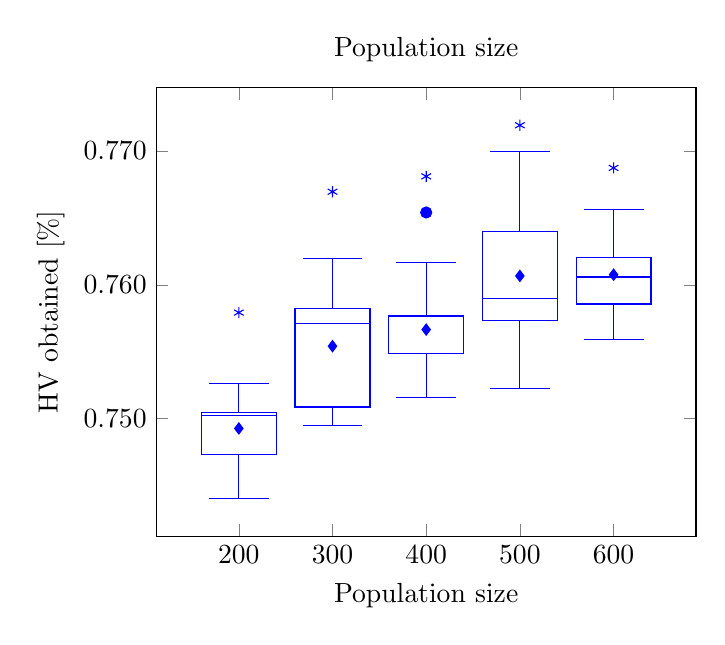
\begin{tikzpicture} 
\begin{axis}[ 
title={Population size}, 
boxplot/draw direction=y, 
xtick={1,2,3,4,5}, 
xticklabels={200,300,400,500,600}, 
x tick label style={rotate=0, align=center}, 
xlabel={Population size}, 
y tick label style={/pgf/number format/.cd,fixed,precision=3, zerofill}, 
ylabel={HV obtained [\%]}, 
] 

% ############## Pop_size=200 ################## 
\addplot[boxplot, mark=*, 
boxplot prepared={ 
lower whisker=0.74401, 
upper whisker=0.75264, 
lower quartile=0.74733, 
upper quartile=0.75048, 
median=0.75022, 
average=0.74927}, 
color = blue, solid, area legend] 
coordinates {}; 
\addplot[only marks,mark=asterisk,color = blue]coordinates{(1,0.75793)}; 

% ############## Pop_size=300 ################## 
\addplot[boxplot, mark=*, 
boxplot prepared={ 
lower whisker=0.74952, 
upper whisker=0.76197, 
lower quartile=0.75087, 
upper quartile=0.75824, 
median=0.75708, 
average=0.75542}, 
color = blue, solid, area legend] 
coordinates {}; 
\addplot[only marks,mark=asterisk,color = blue]coordinates{(2,0.76696)}; 

% ############## Pop_size=400 ################## 
\addplot[boxplot, mark=*, 
boxplot prepared={ 
lower whisker=0.75159, 
upper whisker=0.76165, 
lower quartile=0.75488, 
upper quartile=0.75774, 
median=0.75764, 
average=0.75666}, 
color = blue, solid, area legend] 
coordinates {
(3,0.76541)}; 
\addplot[only marks,mark=asterisk,color = blue]coordinates{(3,0.76811)}; 

% ############## Pop_size=500 ################## 
\addplot[boxplot, mark=*, 
boxplot prepared={ 
lower whisker=0.75223, 
upper whisker=0.76995, 
lower quartile=0.75736, 
upper quartile=0.76401, 
median=0.75898, 
average=0.76067}, 
color = blue, solid, area legend] 
coordinates {}; 
\addplot[only marks,mark=asterisk,color = blue]coordinates{(4,0.77193)}; 

% ############## Pop_size=600 ################## 
\addplot[boxplot, mark=*, 
boxplot prepared={ 
lower whisker=0.75595, 
upper whisker=0.76561, 
lower quartile=0.75857, 
upper quartile=0.76202, 
median=0.76059, 
average=0.76076}, 
color = blue, solid, area legend] 
coordinates {}; 
\addplot[only marks,mark=asterisk,color = blue]coordinates{(5,0.76874)}; 

\end{axis}
\end{tikzpicture}
\end{figure} 
\begin{table}
\centering
\caption{Legend for the boxplot.}
\begin{tabular}{ll}
\toprule
 Index &  Name \\
\midrule
     0 &   200 \\
     1 &   300 \\
     2 &   400 \\
     3 &   500 \\
     4 &   600 \\
\bottomrule
\end{tabular}
\end{table}

\end{document}
